\documentclass{standalone}
\usepackage{tikz}
\usepackage{pgfplots}
\pgfplotsset{compat=newest}
\usepackage{amsmath}
\usepackage[american]{circuitikz}
\usepackage{cmbright}

\definecolor{myred}{RGB}{170,0,0}
\definecolor{myblue}{RGB}{0,0,220}
\definecolor{mygreen}{RGB}{0,150,0}
\definecolor{myorange}{RGB}{255,127,0}
\definecolor{mybrown}{RGB}{150,75,0}

\ctikzset{bipoles/resistor/height=0.2}
\ctikzset{bipoles/resistor/width=0.5}

\begin{document}
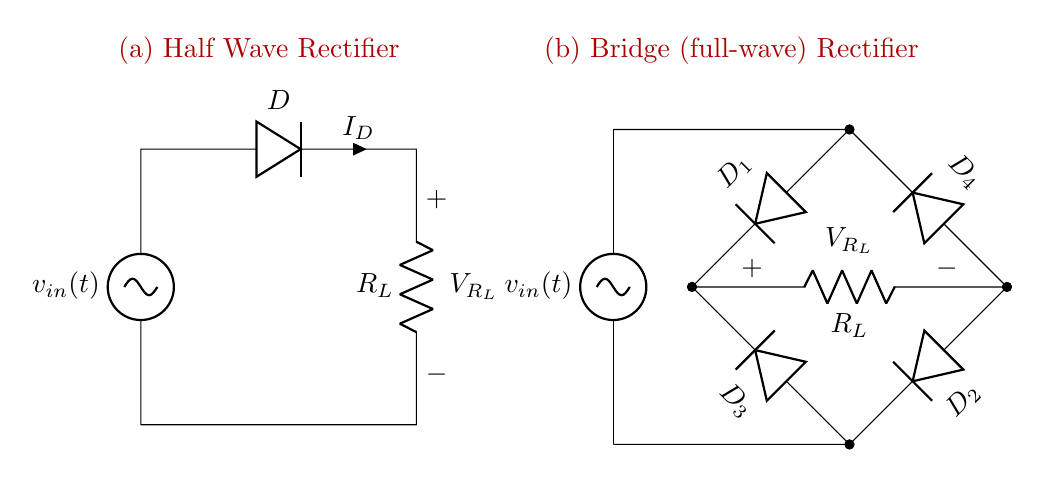
\begin{tikzpicture}
    % Half-wave rectifier circuit
    \begin{scope}
        \node[anchor=center, color=myred, align=center] at (1.5, 3.75) {(a) Half Wave Rectifier};
        \draw (0, -1.0)
            to[sV, l=$v_{in}(t)$] ++(0, 3.5)
            to[D, l=$D$, i^>=$I_D$] ++(3.5, 0)
            to[R, l_=$R_L$, v^={$V_{R_L}$}] ++(0, -3.5)
            to ++(-3.5, 0);
    \end{scope}

    % Bridge rectifier circuit
    \begin{scope}[xshift=6cm]
        \node[anchor=center, color=myred, align=center] at (1.5, 3.75) {(b) Bridge (full-wave) Rectifier};
        % AC voltage source
        \draw (0, -1.25)
            to[sV, l=$v_{in}(t)$] (0, 2.75);

        % Diodes and load resistor
        \draw (0, 2.75)
            to[short] ++(3.0, 0)
            to[D, *-*, l_={$D_1$}] ++(-2.0, -2.0)
            to[R, l_={$R_L$}, v^={$V_{R_L}$}] ++(4, 0)
            to[D, *-*, l={$D_2$}] ++(-2, -2)
            to[short] (0, -1.25);
        \draw (3.0, -1.25)
            to[D, *-*, l={$D_3$}] ++(-2.0, 2.0);
        \draw (5.0, 0.75)
            to[D, *-*, l_={$D_4$}] ++(-2.0, 2.0);
    \end{scope}
\end{tikzpicture}
\end{document}